\subsection{Results}
\label{sec:tweets-svm-results}

The SVMs have an average accuracy of 77.0~\% and an mean (macro-averaged) F$_1$-score of 74.8~\%.

\begin{figure}[htbp]
    \centering
    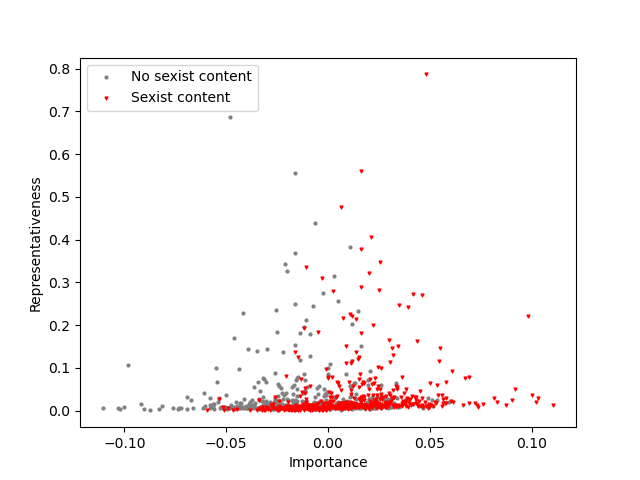
\includegraphics[width=0.9\textwidth]{figures/4-tweets/importance-rep-all-mean-unscaled.png}
    \caption[Representativeness values by LIME importance scores for features in the Twitter data]{Representativeness values by LIME importance scores.}
    \label{fig:tweets-rep}
\end{figure}
\begin{figure}[htbp]
    \centering
    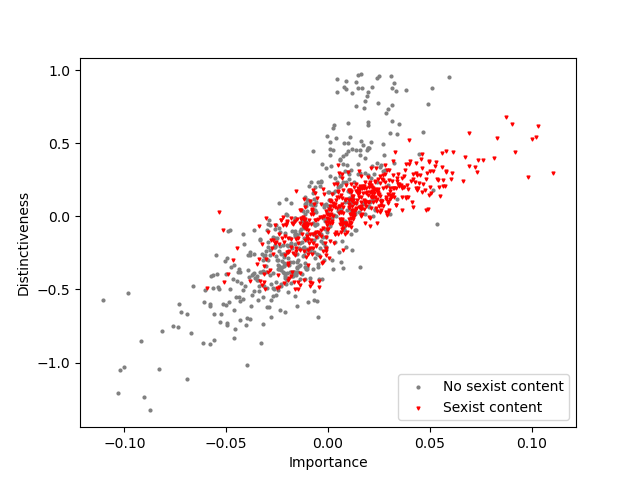
\includegraphics[width=0.9\textwidth]{figures/4-tweets/importance-dist-all-mean-unscaled.png}
    \caption[Distinctiveness values by LIME importance scores for features in the Twitter data]{Distinctiveness values by LIME importance scores.}
    \label{fig:tweets-dist}
\end{figure}

As with the dialect experiment, the importance scores and representativeness scores are (almost) independent of one another (\autoref{fig:tweets-rep}).
The correlation efficient between the two scores is 0.03 for importance values both for tweets with and without sexist content.
Most features that appear especially often in either of the tweet types have importance scores that are close to zero.

By contrast, as \autoref{fig:tweets-dist} shows, the distinctiveness scores and the LIME importance values show a clear correlation: the higher the importance score of a feature is for a given label, the more specific it is to samples with that (gold standard) label.
For both labels, the correlation coefficient for importance and distinctiveness is 0.8.
Importance scores for the group of tweets with sexist content are generally slightly higher than those for features in non-sexist tweets (see also \autoref{fig:tweets-dist}).

\begin{table}[htbp]
    \centering
\begin{tabular}{llrlrl}
\toprule
& & \multicolumn{2}{l}{\textbf{Sexist content}} & \multicolumn{2}{l}{\textbf{No sexist content}} \\
\midrule
{\hashtag} && {\cellcolor[HTML]{92D3B3}0.07} & {\hashtag} & {\cellcolor[HTML]{EEA8A3}-0.07} & {\hashtag} \\
{\hashtag} && {\cellcolor[HTML]{92D3B3}0.07} & {\hashtag} & {\cellcolor[HTML]{EEA8A3}-0.07} & {\hashtag} \\
ou & `or' &  &  &  &  \\
le & `the' &  &  &  &  \\
retour & `return' &  &  &  &  \\
des & `of the' &  &  &  &  \\
" & &{\cellcolor[HTML]{91D3B3}0.07} & \ngram{"\eow} & {\cellcolor[HTML]{EEA8A3}-0.07} & \ngram{"\eow} \\
pater && {\cellcolor[HTML]{A5DBC1}0.05} & \ngram{pa\mow} & {\cellcolor[HTML]{F2BAB6}-0.05} & \ngram{pa\mow} \\
familias &  &  &  &  \\
" && {\cellcolor[HTML]{91D3B3}0.07} & \ngram{"\eow} & {\cellcolor[HTML]{EEA8A3}-0.07} & \ngram{"\eow} \\
autant  & `as much as' & {\cellcolor[HTML]{F2BAB6}-0.05} & \ngram{autant\eow} & {\cellcolor[HTML]{ABDDC5}0.05} & \ngram{autant\eow} \\
dire  & `saying'&  &  &  &  \\
la & `the' &  &  &  &  \\
négation  & `negation'&  &  &  &  \\
radicale & `radical' &  &  &  &  \\
du & `of the' &  &  &  &  \\
féminisme  & `feminism'& {\cellcolor[HTML]{57BB8A}0.11} & \ngram{féminisme\eow{}} & {\cellcolor[HTML]{E67C73}-0.11} & \ngram{féminisme\eow{}} \\
par & `by' &  &  &  &  \\
ces & `these' & {\cellcolor[HTML]{ABDDC5}0.05} & \ngram{ces\eow{}} & {\cellcolor[HTML]{F1B8B3}-0.05} & \ngram{ces\eow{}} \\
spécialistes & `specialists' &  &  &  &  \\
de & `of' &  &  &  &  \\
l' & `the' &  &  &  &  \\
égalité  & `equality'& {\cellcolor[HTML]{5EBE8F}0.10} & \ngram{égalité\eow{}} & {\cellcolor[HTML]{E68078}-0.10} & \ngram{égalité\eow{}} \\
\bottomrule
\end{tabular}
    \caption[Local importance scores for a sample tweet]
    {Local importance scores for a sample tweet.
    Features with importance scores between -0.05 and +0.05 are omitted to preserve space.
    (Continued in the following table.)}
    \label{tab:results-tweets-sample-1}
\end{table}
\begin{table}[htbp]
    \centering
\begin{tabular}{llrlrl}
\toprule
& & \multicolumn{2}{l}{\textbf{Sexist content}} & \multicolumn{2}{l}{\textbf{No sexist content}} \\
\midrule
femme & `woman' & {\cellcolor[HTML]{57BB8A}0.11} & \ngram{femme\eow{}} & {\cellcolor[HTML]{E67C73}-0.11} & \ngram{femme\eow{}} \\
- &  &  &  &  \\
homme  & `man'& {\cellcolor[HTML]{7DCBA5}0.08} & \ngram{homme\eow{}} & {\cellcolor[HTML]{EB9992}-0.08} & \ngram{homme\eow{}} \\
, &  &  &  &  \\
qu' & `what' &  &  &  &  \\
en & `of it' &  &  &  &  \\
pense & `thinks' &  &  &  &  \\
Marlène &  &  &  &  \\
Schiappa &  &  &  &  \\
? &  &  &  & \\
\bottomrule
\end{tabular}
    \caption[Local importance scores for a sample tweet (continued)]
    {(Continuation of the previous table.)
    Local importance scores for a sample tweet.
    Features with importance scores between -0.05 and +0.05 are omitted to preserve space.}
    \label{tab:results-tweets-sample-2}
\end{table}

Tables~\ref{tab:results-tweets-sample-1} and~\ref{tab:results-tweets-sample-2} show the local importance scores for the tweet from Example~\ref{gloss:tweet-preprocessing}.
Since this is a binary classification task, each feature has the same absolute importance scores for both labels---only the sign is inverted.

\begin{figure}[htbp]
    \centering
    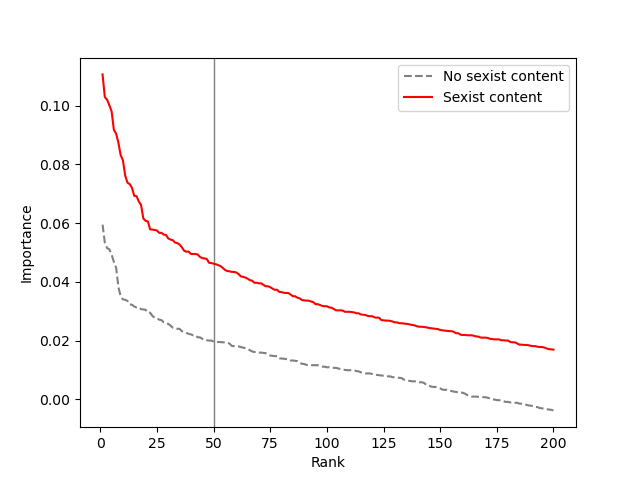
\includegraphics[width=0.9\textwidth]{figures/4-tweets/importance-rank-all-mean-unscaled-50.png}
    \caption[Importance scores for the 200 highest-ranking tweets per label]{Importance scores for the 200 highest-ranking tweets per label.}
    \label{fig:tweets-ranks}
\end{figure}

In the following, I examine patterns into which the top 50 most important features per label fit.
This cut-off point was also chosen to include most of the features with comparatively high importance scores while still retaining a large enough group in order to find patterns within this sub-selection.
\autoref{fig:tweets-ranks} shows the importance scores for the highest-ranking features in both label classes.
The 200 highest-ranking features per class can be found at \url{https://github.com/verenablaschke/ma-thesis/tree/main/models/tweets}.


\subsubsection{Words relating to gender}

\begin{table}[htbp]
    \centering
\begin{tabular}{llrrrl}
\toprule
\textbf{Group} & \textbf{Feature} & \multicolumn{1}{l}{\textbf{Imp.}} & \multicolumn{1}{l}{\textbf{Rep.}} & \multicolumn{1}{l}{\textbf{Dist.}} & \textbf{LIME?} \\
\midrule
\multirow{10}{*}{\begin{tabular}[c]{@{}l@{}}Sexist\\ content\end{tabular}} & \ngram{filles} `girls' & 0.20 & 0.02 & 0.55 &  \ngram{filles\eow}\\
 & \ngram{sexes} `sexes' & 0.20 & 0.01 & 0.39 &  \\
 & \ngram{femmes} `women' & 0.19 & 0.12 & 0.20 &  \ngram{femmes\eow}\\
 & \ngram{sexe} `sex' & 0.16 & 0.01 & 0.18 &  \\
 & \ngram{garçons} `boys'& 0.12 & 0.01 & 0.60 &  \\
 & \ngram{dame} `lady' & 0.10 & 0.00 & 0.02 & \\
 & \ngram{féminin} `feminine, female' & 0.09 & 0.01 & 0.07 & \\
 & \ngram{mecs} `guys' & 0.09 & 0.01 & 0.74 & \\
 & \ngram{fille} `girl' & 0.09 & 0.03 & 0.03 & \ngram{fille\eow}\\
 & \ngram{femme} `woman' & 0.09 & 0.23 & 0.26 & \ngram{femme\eow}\\
 \bottomrule
\end{tabular}
    \caption
    [Features with the top 50 highest LIME scores per label relating to gender]
    {Features with the top 50 highest LIME scores per label that are related to gender.
    The middle columns contain importance, representativeness and distinctiveness scores.
    The context column lists the most frequent word in which each token appears (along with the relative frequency of this word being the origin).
    }
    \label{tab:gender-words}
\end{table}

Many of the tokens that appear in tweets with sexist content and that have high importance scores relate to gender in some way (\autoref{tab:gender-words}).
Most of these are words or subtokens of words that describe women (\textit{filles} `girls,' \textit{femme(s)} `woman/women,' \textit{meuf(s)} `woman/women (colloq.)' and \textit{elles} `they.\textsc{fem}'),\footnote{%
The latter does not always refer to groups of women, it substitutes any plural noun phrase that is grammatically feminine.}
although two words for men also make it into the top 50 (\textit{homme} `man,' \textit{mec} `guy').
Notably, the class of tweets without sexist content also contains one high-importance token referring to women, which is the singular form of one of the aforementioned features: \textit{fille} `girl.' 
However, this word actually appears marginally less often in tweets with this label as one would a randomly distributed feature expect to appear.

\subsubsection{Words relating to feminism and sexism}

\begin{table}[htbp]
    \centering
\begin{tabular}{llrrrl}
\toprule
\textbf{Label} & \textbf{Feature} & {\textbf{Imp.}} & {\textbf{Rep.}} & {\textbf{Dist.}} & \textbf{Context} \\
\midrule
\multirow{4}{*}{\begin{tabular}[c]{@{}l@{}}Sexist\\ content\end{tabular}} & \ngram{féminisme\eow} & 0.11 & 0.01 & 0.30 & féminisme(1.0) `feminism' \\
 & \ngram{égalité\eow} & 0.08 & 0.03 & 0.40 & égalité(1.0) `equality'\\
 & \ngram{sexiste\eow} & 0.06 & 0.02 & 0.25 & sexiste(1.0) `sexist' \\
 & \ngram{féministe\eow} & 0.06 & 0.03 & 0.21 & féministe(1.0) `feminist'\\
 \midrule
\begin{tabular}[c]{@{}l@{}}No sexist\\ content\end{tabular} & \ngram{sexisme\eow} & 0.03 & 0.06 & 0.35 & sexisme(1.0) `sexism'\\
\bottomrule
\end{tabular}
    \caption
    [Features with the top 50 highest LIME scores per label relating to feminism or sexism]
    {Features with the top 50 highest LIME scores per label that are directly related to feminism or sexism.
    The middle columns contain importance, representativeness and distinctiveness scores.
    The context column lists the most frequent word in which each token appears (along with the relative frequency of this word being the origin).
    }
    \label{tab:feminism-sexism}
\end{table}

Several of the features with high importance scores are connected to discussions of feminism or sexism.
Here, tokens relating to feminism or equality are indicators of tweets with sexist content, while the features mentioning sexism are split: \ngram{sexiste\eow} `sexist' is an indicator for sexist content whereas \ngram{sexisme\eow} `sexism' has a high importance score for tweets with \textit{no} sexist content (\autoref{tab:feminism-sexism}).

\subsubsection{Gendered insults}

\begin{table}[htbp]
    \begin{tabular}{llrrrl}
\toprule
\textbf{Label} & \textbf{Feature} & \multicolumn{1}{l}{\textbf{Imp.}} & \multicolumn{1}{l}{\textbf{Rep.}} & \multicolumn{1}{l}{\textbf{Dist.}} & \textbf{Context} \\
\midrule
\multirow{2}{*}{Sexist content} & \ngram{salope\eow} & 0.08 & 0.02 & 0.53 & salope(1.0) `slut, bitch' \\
 & \ngram{asse\eow} & 0.08 & 0.02 & 0.38 & connasse(0.8) `bitch' \\
 \midrule
No sexist content & \ngram{conne\eow} & 0.03 & 0.01 & 0.02 & conne(1.0) `stupid.\textsc{fem}'\\
\bottomrule
\end{tabular}
    \caption
    [Features with the top 50 highest LIME scores per label that are gendered insults]
    {Features with the top 50 highest LIME scores per label that are (subtokens) of insults directed at women.
    The middle columns contain importance, representativeness and distinctiveness scores.
    The context column lists the most frequent word in which each token appears (along with the relative frequency of this word being the origin).
    }
    \label{tab:insults}
\end{table}


Two of the high-ranking features of tweets with sexist contents are (subtokens of) insults directed at women: \ngram{salope\eow} `slut, bitch' and \ngram{asse\eow}, which almost always appears as the suffix of \textit{connasse} `bitch' in this dataset.
However, one of the top 50 indicators of a non-sexist tweet is also such a term: \textit{conne} `bitch; stupid.\textsc{fem}'
Both of the features with high importance scores for the sexist class have high distinctiveness scores, whereas \textit{conne} only occurs in the tweets without sexist content roughly as often as one would expect by chance (see \autoref{tab:insults}).

The presence of insults that either relate to intellectual deficits or that pertain to sexuality fits with the observations that \citet{dupre2020violences} made in a qualitative analysis of sexist tweets.

\subsubsection{Female politicians}

\begin{table}[htbp]
    \centering
\begin{tabular}{llrrrl}
\toprule
\textbf{Label} & \textbf{Feature} & \multicolumn{1}{l}{\textbf{Imp.}} & \multicolumn{1}{l}{\textbf{Rep.}} & \multicolumn{1}{l}{\textbf{Dist.}} & \textbf{Context} \\
\midrule
\multirow{9}{*}{\begin{tabular}[c]{@{}l@{}}No sexist\\ content\end{tabular}} & \ngram{Ségolène\eow} & 0.05 & 0.03 & 0.88 & Ségolène(1.0)  \\
 & \ngram{Christiane\eow} & 0.05 & 0.03 & 0.77 & Christiane(1.0)  \\
 & \ngram{Royal\eow} & 0.04 & 0.03 & 0.87 & Royal(1.0)  \\
 & \ngram{Angela\eow} & 0.03 & 0.06 & 0.86 & Angela(1.0)  \\
 & \ngram{Theresa\eow} & 0.03 & 0.03 & 0.91 & Theresa(1.0)  \\
 & \ngram{Christine\eow} & 0.03 & 0.02 & 0.77 & Christine(1.0)  \\
 & \ngram{Taubira\eow} & 0.03 & 0.03 & 0.74 & Taubira(1.0)  \\
 & \ngram{Lagarde\eow} & 0.02 & 0.01 & 0.78 & Lagarde(1.0)  \\
 & \ngram{May\eow} & 0.02 & 0.03 & 0.89 & May(1.0) \\
 \bottomrule
\end{tabular}
    \caption
    [Features with the top 50 highest LIME scores per label that are names of female politicians]
    {Features with the top 50 highest LIME scores per label that are names of female politicians.
    The middle columns contain importance, representativeness and distinctiveness scores.
    The context column lists the most frequent word in which each token appears (along with the relative frequency of this word being the origin).
    }
    \label{tab:politicians}
\end{table}

Many of the features with high importance scores for the tweets without sexist content are the first and last names of several influential female politicians (Ségolène Royal, Christiane Taubira, Christine Lagarde, Angela Merkel and Theresa May).
While none of these names appear in an especially high proportion of the non-sexist tweets, all them them appear almost exclusively in this class (\autoref{tab:politicians}).

\subsubsection{Pronouns}

\begin{table}[htbp]
    \centering
\begin{tabular}{llrrrl}
\toprule
\textbf{Label} & \textbf{Feature} & \multicolumn{1}{l}{\textbf{Imp.}} & \multicolumn{1}{l}{\textbf{Rep.}} & \multicolumn{1}{l}{\textbf{Dist.}} & \textbf{Context} \\
\midrule
\multirow{10}{*}{\begin{tabular}[c]{@{}l@{}}Sexist\\ content\end{tabular}} & \ngram{t'\eow} & 0.10 & 0.04 & 0.53 & t'(1.0) `your.\textsc{sg}' \\
 & \ngram{te\eow} & 0.09 & 0.05 & 0.44 & te(0.8)  `you.\textsc{sg.acc}'\\
 & \ngram{ta\eow} & 0.06 & 0.02 & 0.26 & ta(0.9) `your.\textsc{sg}'  \\
 & \ngram{tes\eow} & 0.06 & 0.02 & 0.45 & tes(0.6) `your.\textsc{sg}'  \\
 & \ngram{ton\eow} & 0.06 & 0.03 & 0.31 & ton(1.0) `your.\textsc{sg}'  \\
 & \ngram{me\eow} & 0.06 & 0.07 & 0.31 & me(0.9) `me'  \\
 & \ngram{moi\eow} & 0.06 & 0.04 & 0.34 & moi(1.0) `I, me' \\
 & \ngram{ma\eow} & 0.05 & 0.04 & 0.25 & ma(1.0) `my' \\
 & \ngram{toi\eow} & 0.05 & 0.02 & 0.37 & toi(1.0) `you' \\
 & \ngram{mes\eow} & 0.05 & 0.01 & 0.16 & mes(0.9) `my'\\
 \bottomrule
\end{tabular}
    \caption
    [Features with the top 50 highest LIME scores per label that are personal pronouns]
    {Features with the top 50 highest LIME scores per label that are personal pronouns.
    The middle columns contain importance, representativeness and distinctiveness scores.
    The context column lists the most frequent word in which each token appears (along with the relative frequency of this word being the origin).
    }
    \label{tab:tweets-pronouns}
\end{table}

As \autoref{tab:tweets-pronouns} shows, ten of the 50 features with the highest importance scores for the tweets with sexist contents are first and second person singular (informal) pronouns, and these features do indeed also have high distinctiveness scores for that class.
No personal pronouns are included in the top 50 features for the other label.
The fact that so many first and second person pronouns are indicators for sexist content fits the definition of two of the subcategories within that class in the corpus: tweets with sexist content that is \textit{directed} at someone often include second person pronouns by their nature, and tweets \textit{reporting} encounters with sexism often contain first person pronouns (or second person pronouns, if they include direct quotations).

\subsubsection{Punctuation}

Four of the features that LIME deems indicative of sexist content consist of punctuation marks (\ngram{—\eow}, \ngram{...\eow}, \ngram{=\eow} and \ngram{?\mow}), as does one of the high-ranking features of the other class (\ngram{,\mow}).\footnote{%
This should not be confused with the more common comma feature \ngram{,\eow}.
The above-mentioned feature is much rarer and appears in character sequences such as \textit{,''} where it is followed by other letters (usually other punctuation marks).
}
% Of these, the em-dash has the highest distinctiveness score  (0.62), although it is not obvious...
